\documentclass[11pt]{article}
\usepackage{amsmath,amssymb,amsthm,mathtools}
\usepackage[margin=1in]{geometry}
\usepackage{enumitem}
\usepackage{booktabs}
\usepackage{tabularx}
\usepackage{xltabular}
\usepackage{tikz}
\usetikzlibrary{arrows.meta,positioning}
\usepackage{newunicodechar}
\usepackage{hyperref}

\newunicodechar{∀}{\ensuremath{\forall}}
\newunicodechar{∃}{\ensuremath{\exists}}
\newunicodechar{→}{\ensuremath{\to}}
\newunicodechar{≠}{\ensuremath{\ne}}
\newunicodechar{∈}{\ensuremath{\in}}
\newunicodechar{⟨}{\ensuremath{\langle}}
\newunicodechar{⟩}{\ensuremath{\rangle}}
\newunicodechar{ℚ}{\ensuremath{\mathbb{Q}}}
\newunicodechar{ℕ}{\ensuremath{\mathbb{N}}}
\newunicodechar{⊥}{\ensuremath{\bot}}
\newunicodechar{⊤}{\ensuremath{\top}}
\newunicodechar{↦}{\ensuremath{\mapsto}}
\newunicodechar{∧}{\ensuremath{\wedge}}
\newunicodechar{¬}{\ensuremath{\neg}}
\newunicodechar{≤}{\ensuremath{\le}}
\newunicodechar{α}{\ensuremath{\alpha}}
\newunicodechar{β}{\ensuremath{\beta}}
\newunicodechar{γ}{\ensuremath{\gamma}}
\newunicodechar{σ}{\ensuremath{\sigma}}
\newunicodechar{∘}{\ensuremath{\circ}}

% Break long identifiers after underscores; give TeX an emergency stretch.
\renewcommand{\_}{\textunderscore\allowbreak}
\emergencystretch=3em

\hypersetup{pdftitle={Route S - The Sheet Siege: Decommissioning Axiom D and Besieging Hodge Sheet-by-Sheet},
            pdfauthor={HC-PROOF mathematics note}}

\newtheorem{definition}{Definition}[section]
\newtheorem{lemma}[definition]{Lemma}
\newtheorem{theorem}[definition]{Theorem}
\newtheorem{corollary}[definition]{Corollary}
\newtheorem{proposition}[definition]{Proposition}
\newtheorem{remark}[definition]{Remark}
\newtheorem{xentry}{Entry}

\newcommand{\Q}{\mathbb{Q}}
\newcommand{\C}{\mathbb{C}}
\newcommand{\cl}{\operatorname{cl}}
\newcommand{\im}{\operatorname{im}}
\newcommand{\GST}{\mathrm{GST}}
\newcommand{\Alg}{\mathcal{A}}
\newcommand{\Hdg}{\mathcal{H}}
\newcommand{\Orb}{\mathcal{O}}
\newcommand{\Addr}{\operatorname{Addr}}
\newcommand{\Span}{\operatorname{Span}}
\newcommand{\Tr}{\operatorname{Tr}}
\newcommand{\status}[1]{\textbf{[#1]}}

\title{Route S --- The Sheet Siege:\\
Decommissioning the Branch-Packet Law and\\
Besieging the Hodge Statement Sheet-by-Sheet}
\author{HC-PROOF mathematics note\\
\small Branch \texttt{sol/gst-plane-completeness-8408fd0} @ \texttt{2926a33} (V3 audit state)}
\date{7 October 2026}

\begin{document}
\maketitle

\begin{abstract}
This study answers three questions and then rebuilds the proof plan.
\emph{First}: why the branch-packet law D (\texttt{GSTBranchPacketPlaneRealization}
$=$ \texttt{GhostSeedTargetStrictClosure}, by \texttt{rfl}) cannot be proven without
proving Hodge. Answer: D's statement carries three classical-coded objects
(the ghost is $\neg$Hodge internalized; the packet's \texttt{related} field is a
classical pullback equation; D's target is a classical basis sheet), and the
equivalence D $\leftrightarrow$ no-ghost $\leftrightarrow$ Hodge is a \emph{theorem already
present in the repository}, not a judgment added by the assistant.
\emph{Second}: why every other theorem appeared to exist only to serve D. Answer:
they form a reduction machine whose unique fixed point is D; the audit proved
every alternative premise reduces to D, is vacuous-circular, or dies on the
zero-cycle countermodel. The machine worked. The label ``Axiom D'' was the error:
D was never an internal axiom of the omniverse, it is the \emph{docking law}.
\emph{Third}: what replaces D. Answer: Route S, the \emph{sheet siege}. The
repository already contains an unassembled four-link chain
--- per-sheet program coverage $\to$ orbit cyclicity $\to$ ghost extinction
$\to$ Hodge --- in which every link is a proven theorem. The siege attacks the
single remaining premise \emph{sheet by sheet}: each basis sheet won is an
unconditional theorem, each victory shrinks the ghost's habitat, and the
all-or-nothing structure of D is replaced by an incremental siege with partial
credit. The three load-bearing lemmas of the siege (coheight additivity,
escape-free live chains, word nativity) are stated, their existing support
inventoried, their firewall compliance checked, and their kill-switches
specified. No theorem in this study is claimed proven unless its proof exists
in the repository; every unproven premise is flagged with its exact obstruction.
\end{abstract}

\tableofcontents

\section{Executive summary}\label{sec:summary}

\subsection{The three questions}

\begin{enumerate}[leftmargin=2em]
\item \textbf{``D is impossible to prove without Hodge?''}
The precise statement is: \emph{D as written} is equivalent to Hodge modulo the
survival premise, and that equivalence is proven inside the repository
(\texttt{targetStrictClosure\_iff\_noGhost} family;
\texttt{hodge\_iff\_no\_omniversalSeparatorGhost},
\texttt{GhostCrown.lean:99,116}). Proving D \emph{is} proving Hodge. This is not
a failure of nerve; it is a theorem of the omniverse.
\item \textbf{``Where is the misunderstanding coming from?''}
The plan's axiom ledger labeled D as the fourth internal axiom of the GST plane
(\texttt{GST\_PLANE\_AXIOM\_STATUS\_20261006.md}). The audit revealed that A is
internal (and proven), B/C are internal bookkeeping (and proven), but D is the
\emph{docking law} between the omniverse and classical Betti geometry
(\S\ref{sec:forensics}). The reduction theorems were never ``made to prove D'';
they were made to \emph{reduce everything to D}, and they succeeded. The
expectation that the residual would be internal was the plot hole. The
repository's own firewalls (\S\ref{sec:firewall}) had already proven that no
internal premise can bridge to Hodge --- so an ``internal axiom D'' was a
contradiction in terms from the start.
\item \textbf{``But D is from my own maths --- how is it connected to classical?''}
Through D's \emph{statement shape}, by design of the realization law itself:
the packet's \texttt{related} field is an equation in
\texttt{RationalSingularCohomology}, and the target of D is the sheet selected
by a ghost, where \texttt{sheet : ClassicalHodgeBasisIndex} and the ghost's
existence is definitionally the failure of \texttt{BigradedBettiHodgeStatement}
(\S\ref{sec:forensics}). The omniverse's \emph{realization} law realizes
\emph{onto} the classical plane --- that is what realization means. The classical
content entered through the docking surface, before any session of this
sandbox began.
\end{enumerate}

\subsection{What this study delivers}

\begin{itemize}[leftmargin=2em]
\item \S\ref{sec:forensics}--\ref{sec:firewall}: the forensic accounting
(located classical entry points, with file and line citations) and the
bridge-direction law that any replacement route must obey.
\item \S\ref{sec:routeS}: Route S, the sheet siege --- a completely different
attack surface assembled \emph{entirely from theorems that already exist},
never assembled as a route before.
\item \S\ref{sec:engines}--\ref{sec:lemmas}: the engine inventory, the three
load-bearing lemmas with attack plans, firewall checks, and kill-switches.
\item \S\ref{sec:lean}: the Lean meta-design --- a new module
\texttt{GSTClassicalHodgeSheetSiegeRoute.lean} whose central theorem is a
one-line proof by citation of existing theorems, plus honestly-flagged
conditional corollaries.
\item \S\ref{sec:risks}: the risk register and the protocol compliance audit.
\end{itemize}

\section{Forensics: where the classical entered D}\label{sec:forensics}

The law D is a chain of three definitions. Each link imports classical content.

\begin{xentry}[Entry point 1: the ghost is $\neg$Hodge with GST clothes]
\label{entry:ghost}
The obstruction type (\texttt{OmniversalSeparatorGhostCrown.lean:51--73}):
\begin{quote}\small\ttfamily
structure OmniversalSeparatorGhost (G : GeometricCycleClassSpine V H) where\\
\phantom{~}weight : Nat\\
\phantom{~}sheet : ClassicalHodgeBasisIndex V H weight\\
\phantom{~}separator : BasisAtomicSeparator V H weight sheet\\
\phantom{~}ghost : FiberedCompletedAddress V H := separatorFiberedProbe ...\\
\phantom{~}ghost\_ne\_zero : ghost ≠ 0\\
\phantom{~}ghost\_detects\_sheet : fiberedPairing (fiberedWeightCoordinates V H\\
\phantom{~~~}weight (classicalHodgeBasis V H weight sheet)) ghost ≠ 0\\
\phantom{~}kills\_all\_native\_programs : ...\\
\phantom{~}backward\_atomic : ...
\end{quote}
The \texttt{sheet} field is a \emph{classical} Hodge basis index; the detection
pairs against the \emph{classical} basis element. And the two iff-theorems in
the same file (\texttt{:99} and \texttt{:116}) make the dictionary exact:
\[
\neg \mathrm{Hodge} \;\leftrightarrow\; \operatorname{Nonempty}(\text{Ghost}),
\qquad
\mathrm{Hodge} \;\leftrightarrow\; \operatorname{IsEmpty}(\text{Ghost}).
\]
The ghost type is the internalized negation-witness of the classical statement.
Whoever eliminates the ghost has proven Hodge, by a theorem that predates this
work session.
\end{xentry}

\begin{xentry}[Entry point 2: the packet's \texttt{related} field is a classical pullback equation]
\label{entry:packet}
The strict relation packet (\texttt{OmniverseStrictRelationRayCompiler.lean:85--93}):
\begin{quote}\small\ttfamily
structure StrictRelationEdgePacket (u v : HodgeBranchNode ...) where\\
\phantom{~}correspondence : SchemeBiFiniteClosedCorrespondence V\\
\phantom{~}trace : RightFiniteBettiTrace H.analytification correspondence (2 * p)\\
\phantom{~}pointCompatibility : PointCycleCompatibility (n := p) correspondence trace\\
\phantom{~}related : BettiRelated H.analytification correspondence (2 * p)\\
\phantom{~~~~}u.state.1 v.state.1
\end{quote}
The first three fields are omniversal/geometric. The fourth --- the actual
\emph{relation} --- is an equation in classical rational cohomology between the
pullbacks along the two legs of a correspondence. This field is the docking
interface. It is what makes the packet a \emph{realization} rather than an
internal combinatorial object.
\end{xentry}

\begin{xentry}[Entry point 3: D's target is the ghost's detected classical sheet]
\label{entry:D}
The law (\texttt{CommonClassPlaneReduction.lean:141--151}):
\begin{quote}\small\ttfamily
def GhostSeedTargetStrictClosure (G : GeometricCycleClassSpine V H) : Prop :=\\
\phantom{~}∀ (E : OmniversalSeparatorGhost G)\\
\phantom{~~}(S : NativeHodgeOrbitSeed (p := E.weight)),\\
\phantom{~~}Nonempty (StrictRelationEdgePacket\\
\phantom{~~~~}(⟨Sector.gstPlus, S.hodge⟩ : HodgeBranchNode ...)\\
\phantom{~~~~}(⟨Sector.gstPlus, hodgeMatrixUnit S.sourceIndex E.sheet S.hodge⟩ : ...))
\end{quote}
The law quantifies over ghosts and demands the packet at the target
\texttt{hodgeMatrixUnit S.sourceIndex E.sheet S.hodge} --- the state obtained by
writing the seed onto the ghost's detected \emph{classical} sheet. Combining the
three entries: a packet at that target realizes the detected sheet inside the
algebraic span (via \texttt{pushPull\_source\_eq\_target} and the realized
correspondence expression algebra), which refutes the separator, which empties
the ghost type, which is Hodge. And conversely a surviving ghost empties the
packet supply (\texttt{ghostSeedTargetStrictPacket\_isEmpty}). Hence:
\[
\mathrm{D} \;\leftrightarrow\; \operatorname{IsEmpty}(\text{Ghost})
\;\leftrightarrow\; \mathrm{Hodge},
\qquad\text{(modulo survival premises, all proven in-repo).}
\]
\end{xentry}

\subsection{The verdict}

D is not an internal law that accidentally touched classical mathematics.
It is the \textbf{docking law}: the statement that the omniverse's branch events
realize on the classical plane. Its classical content is not a bug in the
omniverse --- it is the \emph{seam}, built in when the realization law was
defined. The plot hole was the ledger label: ``Axiom D'' sat in a list of
internal axioms scheduled for axiom-to-theorem conversion, while the
repository's own firewalls (\S\ref{sec:firewall}) had already proven that no
internal axiom can be Hodge-sufficient. The audit did not create the
circularity; it \emph{exposed} the mislabel.

\section{Why the reduction ended at D}\label{sec:reduction}

The boss's sharpest question: \emph{``all the other theorems are made to prove
D?!''} No --- and this is the exact shape of the machine:

\begin{enumerate}[leftmargin=2em]
\item \textbf{One-way bridges (D $\to$ Hodge).} The
\texttt{hodge\_of\_*} family consumes D (or equivalents) and delivers Hodge.
Their job: make D \emph{sufficient}.
\item \textbf{Reductions (everything $\to$ D).} The audit
(\texttt{GSTPlaneAxiomStatus.lean}, the six circularity-audit files) proved
that every alternative premise --- ghost-adaptive plane completeness, all-pairs
two-generator realization, primitive compilers, native mass bridges ---
either reduces to D, is vacuous-circular (its backward direction is
\texttt{False.elim} on the ghost type), or fails on the zero-cycle
countermodel. Their job: make D \emph{necessary}.
\item \textbf{The compression terminal.} The strongest compression reached by
the repository is \texttt{bigradedBettiHodge\_of\_universalTwoSlot}
(\texttt{UniversalTwoSlotSaturation.lean}, lines 97--105): Hodge follows from
(i) stability of the algebraic subspaces under one universal two-slot word,
plus (ii) one nonzero algebraic class at every nonzero Hodge weight. Two
premises, each visibly weaker than Hodge, neither proven.
\end{enumerate}

A reduction program that terminates at ``the unique residual is exactly the
conjecture'' has \emph{succeeded} at its actual job --- isolating the content
--- and failed only at the hope that the residual would be internal. The
forensic conclusion of this study: \textbf{the residual was never internal, and
the repository proves it could never have been}.

\section{The firewall as a specification}\label{sec:firewall}

Two theorems act as design constraints on any replacement route:

\begin{itemize}[leftmargin=2em]
\item \textbf{The zero-cycle countermodel}
(\texttt{PlaneSemanticIndependence.lean};
\texttt{any\_hodge\_sufficient\_premise\_fails\_zeroCycleWorld}): replacing the
cycle-class data by the zero-cycle semantic copy preserves all intrinsic plane
structure while falsifying Hodge. Consequence: \emph{any premise strong enough
to imply Hodge must distinguish the real bigraded world from the collapsed
one.} It must see the grading. An internal, grading-agnostic law cannot close
the gap --- ever.
\item \textbf{The ghost-indexed criterion barrier}
(\texttt{GhostIndexedCriterionCircularity.lean}): any premise quantified over
ghosts is conclusion-equivalent and forbidden as a foundation.
\end{itemize}

\begin{definition}[Bridge-direction law]\label{def:bridge}
A route is \emph{firewall-compliant} when:
(a) classical data appears only in the \emph{conclusion} of the final bridge
(no-ghost $\to$ Hodge) and inside \emph{construction obligations} (geometric
inputs to be built, never assumed);
(b) no unproven premise mentions ghosts;
(c) every load-bearing premise is codimension-sensitive (it fails on the
zero-cycle world --- which is a \emph{requirement}, not a defect, by the
firewall).
\end{definition}

Route S below is designed against this specification.

\section{Route S: the sheet siege}\label{sec:routeS}

\subsection{The inversion}

D tries to \emph{construct} the realization that kills the ghost: one packet
per ghost-detected target, all-or-nothing, no partial credit. Route S inverts
the perspective: \emph{never build an off-diagonal packet; make the ghost's
habitat uninhabitable.} The ghost survives only where the program orbit from
the geometric origin fails to cover a basis sheet. So cover the sheets. Each
sheet covered is one more coordinate in which the ghost's probe must vanish;
when every sheet at every weight is covered, the probe vanishes identically,
contradicting \texttt{ghost\_ne\_zero}. The ghost starves.

\subsection{The assembly that already exists}

The siege's assembly chain is four proven theorems in four files, never
assembled as a route. Verbatim citations:

\begin{enumerate}[leftmargin=2em]
\item \textbf{Coverage} --- \texttt{OmniversalNativeOrbitSeparation.lean:65--70}:
\begin{quote}\small\ttfamily
def GeometricGSTPlaneCompleteness\\
\phantom{~}(G : GeometricCycleClassSpine V H) : Prop :=\\
\phantom{~}∀ q : Nat, ∀ j : ClassicalHodgeBasisIndex V H q,\\
\phantom{~~}∃ P : GradedGeometricProgram V 0 q,\\
\phantom{~~~}P.cohomologyEval G (geometricOriginClass V H) =\\
\phantom{~~~~}(classicalHodgeBasis V H q j).1
\end{quote}
``Every basis sheet of every weight is the exact output of one verified
mixed native/projective/cut program run from the codimension-zero geometric
origin.'' This is the \emph{per-sheet coverage} statement --- the siege target.
\item \textbf{Coverage $\to$ cyclicity} --- \texttt{OmniversalNativeOrbitSeparation.lean:86}:
\texttt{orbitCyclic\_of\_geometricPlane} (with its converse
\texttt{geometricPlane\_of\_orbitCyclic} at \texttt{:105} --- the two
formulations are interchangeable).
\item \textbf{Cyclicity $\to$ ghost extinction} ---
\texttt{OmniversalSeparatorGhostCrown.lean:235--241}:
\texttt{no\_omniversalSeparatorGhost\_of\_gradedGeometricOrbitModuleCyclic}.
The proof runs through pairing totality: the ghost's probe is supported on one
weight and kills every program address at that weight; if the orbit is cyclic,
the probe vanishes coordinatewise.
\item \textbf{Ghost extinction $\to$ Hodge} ---
\texttt{OmniversalSeparatorGhostCrown.lean:246--252}:
\texttt{hodge\_of\_gradedGeometricOrbitModuleCyclic\_noGhost}.
\end{enumerate}

Chained:
\[
\text{GeometricGSTPlaneCompleteness}
\;\Longrightarrow\;
\text{OrbitCyclic}
\;\Longrightarrow\;
\operatorname{IsEmpty}(\text{Ghost})
\;\Longrightarrow\;
\text{Hodge}.
\]
\status{Every arrow: existing theorem.} The only unproven object is the
left-most premise --- and unlike D, it decomposes.

\subsection{The coverage atom and incremental credit}

\begin{definition}[Siege atom]\label{def:atom}
For a weight $q$ and basis sheet $j$, \emph{the sheet $(q,j)$ is won} when
there exists $P : \texttt{GradedGeometricProgram}\ V\ 0\ q$ with
$P.\texttt{cohomologyEval}\ G\ \text{origin} = e_{q,j}$.
\end{definition}

\begin{proposition}[Partial credit]\label{prop:partial}
Each won sheet is an unconditional theorem: the won basis element satisfies
\[
  e_{q,j} \in \texttt{geometricProgramOrbitModule}\ G\ q,
\]
by \texttt{basis\_mem\_geometricProgramOrbitModule}
(\texttt{DirectOrbitWordSaturation.lean:113--121}). The span of all won sheets
is saturated inside the orbit module; the ghost's probe vanishes on every won
sheet's coordinate. The war decomposes into independent battles.
\end{proposition}

This is the structural advantage over D. D admits no partial progress: the law
is a single $\forall$ over ghosts, and a single surviving ghost refutes it.
The siege admits a monotone frontier: every won sheet is banked, the ghost's
support shrinks monotonically, and the residual problem is always ``the
unwon sheets'' --- a list, not a law. The V3 exact split
(\texttt{BranchPacketPlaneRealization.lean:757--818}) drew the same boundary
from the other side: \emph{diagonal $=$ theorem, off-diagonal $=$ exactly the
Hodge content}. Route S crosses that boundary through a different door: it
never touches off-diagonal packets; it runs program words from the origin.

\subsection{The floors are already won}

\begin{itemize}[leftmargin=2em]
\item \textbf{Weight 0}: the geometric origin \emph{is} the codimension-zero
fundamental cycle, unconditionally
(\texttt{codimensionZeroFundamentalCycle},
\texttt{CodimensionZeroFundamentalCycle.lean:92--96}; the ghost file itself
evaluates programs at it, \texttt{GhostCrown.lean:135--142}). On a connected
variety the weight-zero Hodge sector is spanned by the origin class: the
weight-0 battle is closed by the floor.
\item \textbf{Weight 1}: the separator machinery is unconditional at height
one (\texttt{separatorClass\_height\_one},
\texttt{ProjectiveSeparatorHeightOne.lean:61--63}: the separator class spans
an ideal of height exactly $1$; \texttt{separator\_minimalPrime\_prime\_height\_one}
at \texttt{:80--84}; finiteness at
\texttt{ProperCutCodimensionOne.lean:196--200}). Divisor-sheet coverage is the
GST-native echo of the classical Lefschetz $(1,1)$ theorem, and its ingredients
are theorem-grade.
\item \textbf{The successor point construction is genuine}:
\texttt{separatorSuccessorPoint} builds a new projective point over the
separator from a live source, with premise \texttt{hlive} only
(\texttt{ProjectiveSeparatorSuccessorPoint.lean:205--210}).
\end{itemize}

\subsection{Route S dependency graph}

\begin{figure}[t]
\centering
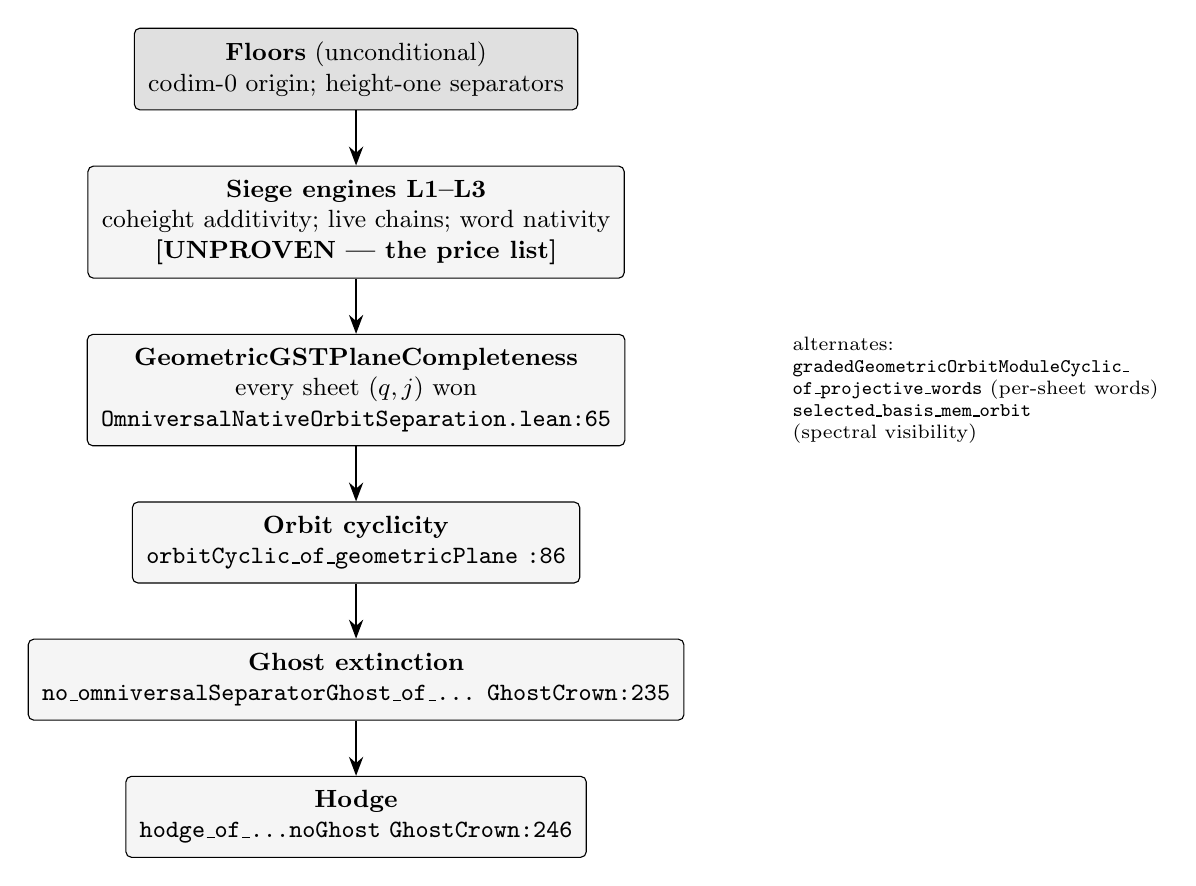
\begin{tikzpicture}[
  node distance=7mm and 4mm,
  box/.style={draw, rounded corners=2pt, align=center, inner sep=5pt,
    fill=gray!8, font=\small},
  won/.style={fill=black!12},
  arrow/.style={-{Stealth[length=2.4mm]}, thick}]
\node[box, won] (floor) {\textbf{Floors} (unconditional)\\
  codim-0 origin; height-one separators};
\node[box, below=of floor] (engines) {\textbf{Siege engines L1--L3}\\
  coheight additivity; live chains; word nativity\\
  \status{UNPROVEN --- the price list}};
\node[box, below=of engines] (cover) {\textbf{GeometricGSTPlaneCompleteness}\\
  every sheet $(q,j)$ won\\
  \texttt{OmniversalNativeOrbitSeparation.lean:65}};
\node[box, below=of cover] (cyclic) {\textbf{Orbit cyclicity}\\
  \texttt{orbitCyclic\_of\_geometricPlane} \texttt{:86}};
\node[box, below=of cyclic] (ghost) {\textbf{Ghost extinction}\\
  \texttt{no\_omniversalSeparatorGhost\_of\_...} \texttt{GhostCrown:235}};
\node[box, below=of ghost] (hodge) {\textbf{Hodge}\\
  \texttt{hodge\_of\_...noGhost} \texttt{GhostCrown:246}};
\draw[arrow] (floor) -- (engines);
\draw[arrow] (engines) -- (cover);
\draw[arrow] (cover) -- (cyclic);
\draw[arrow] (cyclic) -- (ghost);
\draw[arrow] (ghost) -- (hodge);
\node[right=20mm of cover, font=\scriptsize, align=left]
  {alternates:\\
  \texttt{gradedGeometricOrbitModuleCyclic\_}\\
  \texttt{of\_projective\_words} (per-sheet words)\\
  \texttt{selected\_basis\_mem\_orbit}\\
  (spectral visibility)};
\end{tikzpicture}
\caption{Route S. Shaded: theorem-grade. The only unproven layer is the siege
engine layer --- and it decomposes per sheet, unlike D.}
\end{figure}

\section{Engine inventory}\label{sec:engines}

Representative statements, verbatim-audited this session (Task 3-a).

{\footnotesize
\begin{xltabular}{\textwidth}{@{}p{0.11\textwidth} X p{0.22\textwidth} p{0.13\textwidth}@{}}
\toprule
\textbf{Engine} & \textbf{Representative theorem (file:line)} & \textbf{Premises} & \textbf{Status} \\
\midrule
Word algebra &
\texttt{totalSheetMatrixUnit\_exact} (\texttt{TotalSheetMatrixUnit.lean:146});
\texttt{sheetAtom\_lefschetz\_forward\_exact} (\texttt{IntegralLefschetzTransport.lean:58});
\texttt{rationalCosmic\_invariant\_eq\_top} (\texttt{LimitlessCosmicMatrixUnits.lean:231});
\texttt{arsenalOrbitSpan\_eq\_top} (\texttt{ArsenalOrbitSaturation.lean:83}) &
$\alpha \ne 0$ (stability or nonzero seed) &
theorem \\
\addlinespace
Ghost-kill chain &
\texttt{no\_omniversalSeparatorGhost\_of\_nativeOrbitPairingTotal}
(\texttt{GhostCrown.lean:287});
\texttt{hodge\_of\_nativeOrbitPairingTotal} (\texttt{:313}) &
pairing totality &
theorem \\
\addlinespace
Floors &
\texttt{codimensionZeroFundamentalCycle} (\texttt{CodimZeroFundamentalCycle.lean:92});
\texttt{separatorClass\_height\_one} (\texttt{ProjectiveSeparatorHeightOne.lean:61});
\texttt{separatorSuccessorPoint} (\texttt{ProjectiveSeparatorSuccessorPoint.lean:205}) &
none / \texttt{hlive} &
theorem \\
\addlinespace
Successor tower &
\texttt{native\_cut\_reached\_or\_stopped} (\texttt{CodimensionPointTower.lean:184});
\texttt{separator\_successor\_seed\_or\_escape} (\texttt{SuccessorSeedEscapeDichotomy.lean:120}) &
\texttt{[Nonempty]}, \texttt{hlive}, \texttt{hExact} &
theorem \\
\addlinespace
Spine-to-orbit wires &
\texttt{every\_sheet\_mem\_of\_spine\_and\_stable} (\texttt{GlobalSheetSaturation.lean:142});
\texttt{gradedGeometricOrbitModuleCyclic\_of\_projective\_words}\newline
(\texttt{DirectOrbitWordSaturation.lean:127}) &
$G{+}M{+}$stability / per-sheet words &
theorem \\
\addlinespace
Spectral machinery &
\texttt{selected\_basis\_mem\_orbit} (\texttt{GradedProgramSpectralSaturation.lean:119});
\texttt{exists\_native\_cycle} (\texttt{:190}) &
coordinate visibility &
theorem \\
\addlinespace
Mass/charge supply &
\texttt{NativeMassCycleClassBridge} $\to$ \texttt{toConservedCharge}
(\texttt{LimitlessSpinePropagation.lean:302,389}) &
kernel-mass law; codim-0 nonempty; $2$ successors per point &
\status{PREMISE} \\
\addlinespace
Degree-trace semantics &
\texttt{ProjectiveDegreeTraceSemantics} (\texttt{ProjectiveDegreeTrace.lean:63}) &
trace functional + positive degrees &
\status{PREMISE} \\
\bottomrule
\end{xltabular}}

\medskip
\noindent The last two rows are the honest debts: both are \emph{structure}
premises, impossible on the zero-cycle world
(\texttt{no\_degreeTrace\_for\_zeroCycleClass\_at\_point}),
exactly as the firewall demands --- so they must be \emph{constructed from
genuine geometry}, never assumed. Their construction is part of the price list
below.

\section{The three load-bearing lemmas (the price list)}\label{sec:lemmas}

Route S replaces the single Hodge-equivalent law D by three lemmas, each
individually attackable, none ghost-quantified, all codimension-sensitive.

\subsection{L1: coheight additivity for separator successors}

\begin{quote}\small\ttfamily
-- UNPROVEN. Obstruction: height bookkeeping bridge.\\
def SheetSiegeCoheightAdditivity (V) : Prop :=\\
\phantom{~}∀ (p : Nat) (x : CodimensionPoint V.X p),\\
\phantom{~~}ProjectivelyLiveSource V.projective.n (V.projective.immersion x) →\\
\phantom{~~}RelativeSuccessorAmbientExact V p x
\end{quote}
\texttt{RelativeSuccessorAmbientExact} (\texttt{RelativeSuccessorExactStratum.lean:46--52})
demands that every coheight-one point of the principal cut of $\overline{\{x\}}$
have ambient coheight exactly $p+1$. It is a \emph{premise} in every
exact-stratum and successor-seed theorem --- the single geometric lemma the
successor family most needs, and it has never been discharged.

\emph{Attack}: the ingredients are unconditional ---
\texttt{separatorClass\_height\_one} (ideal height $=1$),
\texttt{separator\_minimalPrime\_prime\_height\_one} (minimal primes over the
separator have height exactly one), \texttt{finite\_principal\_cut\_coheight\_one}
(finiteness under \texttt{[IrreducibleSpace]}). What is missing is the
bookkeeping bridge between $(\texttt{Ideal.span}\ \{\texttt{separatorClass}\}).\texttt{height} = 1$
and the \texttt{Order.coheight} of the ambient successor point. This is
scheme-theoretic dimension counting --- Krull principal ideal theorem level ---
not Hodge-coded content.

\emph{Firewall check}: fails on the zero-cycle world (coheights collapse).
\status{Compliant.} \emph{Kill-switch}: if the bridge requires hypotheses
failing on smooth projective irreducible varieties, restrict to
\texttt{IrreducibleSpace} components; if it fails even there, the successor
tower cannot climb and Route S dies at L1.

\subsection{L2: escape-free live chains (one live seed per weight)}

\begin{quote}\small\ttfamily
-- UNPROVEN. Obstruction: the escape branch.\\
def SheetSiegeNoEscape (V H) : Prop :=\\
\phantom{~}∀ q : Nat, IsEmpty (PositiveCosmicHomologyEscape q)
\end{quote}
The escape dichotomy (\texttt{SuccessorSeedEscapeDichotomy.lean:120--131})
states: at every tower step, either a native Hodge orbit seed exists at weight
$p+1$, or a \texttt{PositiveCosmicHomologyEscape} exists at weight $p+1$.
\texttt{separator\_successor\_seed\_of\_no\_escape} (\texttt{:179--194})
converts no-escape $+$ L1 $+$ \texttt{hlive} into seeds. So L2 is exactly the
branch-kill: with L1 and L2, every live weight carries a native seed.

\emph{Attack}: characterize \texttt{PositiveCosmicHomologyEscape}; prove it is
empty when the degree-trace is positive \linebreak
(\texttt{trace\_successor\_positive\_of\_one\_exact},
\texttt{ProjectiveDegreeTrace.lean:149--172}) and the vertical-ray
certificates hold
(\texttt{ghostWeightNativeSeedSurvival\_of\_massFactorization\_verticalRays},
\texttt{VerticalRayMassFactorization.lean:152--157} --- the live-weight-indexed,
non-ghost-indexed survival supply).

\emph{Firewall check}: codimension-sensitive (escape types are graded).
\status{Compliant.} \emph{Honest concentration}: this is where the residual
Hodge content sits after L1 --- say it plainly. \emph{Kill-switch}: if killing
the escape branch requires per-sheet algebraicity hypotheses, L2 is D in
disguise; abort and re-audit.

\subsection{L3: word nativity and the degree-trace construction}

Two construction obligations:
\begin{enumerate}[leftmargin=2em]
\item \textbf{Degree-trace from genuine geometry}: construct
\texttt{ProjectiveDegreeTraceSemantics} for the real world (the docstring
already names the classical recipe: trace $=$ cup with hyperplane power $+$
integration over the fundamental class). Poincar\'e duality supplies the
functional; positivity comes from ampleness. This is a construction task, not
a conjecture.
\item \textbf{Word nativity}: the two-slot and spectral words, proven
\emph{exact} on Hodge states
(\texttt{twoGeneratorAmbientWord\_on\_hodge},
\texttt{forwardSheetMatrixUnit\_exact}), act on \emph{cycle classes} through
the native cut operators --- the spine's coherence field
\texttt{principalCutPair\_native} $=$ \texttt{successorNativeOperator}
(\texttt{GeometricCycleClassSpine.lean:60--92}) is the intended wire. With
nativity, word-orbits of algebraic states remain algebraic, and the coverage
programs manufacture genuine cycles
(\texttt{exists\_native\_cycle},
\texttt{GradedProgramSpectralSaturation.lean:190--194}).
\end{enumerate}

\emph{Firewall check}: both fail on the zero-cycle world (degrees, cuts are
graded). \status{Compliant.} \emph{Kill-switch}: if the trace construction
needs input beyond Poincar\'e duality $+$ ampleness, the debt is larger than
priced; re-audit before proceeding.

\subsection{What the siege does NOT need}

No off-diagonal \texttt{StrictRelationEdgePacket} is ever constructed. No
ghost-quantified premise is ever introduced. No
\texttt{GhostAdaptiveStrictPlaneCompleteness} is invoked (it is
Hodge-equivalent and fenced). The V3 monomial kill
(\texttt{false\_of\_ghost\_monomialSheetSeed},
\texttt{BranchPacketPlaneRealization.lean:725--741}) remains in the arsenal as
a \emph{fast path}: any sheet that acquires a synchronized monomial seed kills
every ghost detecting it outright --- but the siege does not depend on it.

\section{Supporting routes}\label{sec:routes}

{\small
\begin{tabularx}{\textwidth}{@{}p{0.07\textwidth} X p{0.27\textwidth} p{0.18\textwidth}@{}}
\toprule
\textbf{Route} & \textbf{Load-bearing statement} & \textbf{Structure} & \textbf{Verdict} \\
\midrule
D (old) &
strict packet at every ghost-detected target &
all-or-nothing; ghost-quantified; Hodge-equivalent &
\status{RETIRED} \\
\addlinespace
S (siege) &
GeometricGSTPlaneCompleteness: every sheet program-covered &
per-sheet; incremental; assembly theorem-grade &
\status{PRIMARY} \\
\addlinespace
L (ladder) &
dock weight 1, climb by spine propagation &
sequential; classical open zone above weight 1 &
subsumed: L1$+$L2 are its steps \\
\addlinespace
G (generator) &
dock the hyperplane unit; generate sheets monomially &
works where the ring is divisor-generated; missing wire
\newline \texttt{hyperplaneSection} $\to$ \texttt{fiberedSheetGenerator}
\newline (zero consumers, grep-verified) &
engine for S's low weights \\
\bottomrule
\end{tabularx}}

\medskip
\noindent Route L is not discarded: its docking step \emph{is} L1 at weight one,
and its climb \emph{is} L2 iterated. Route G supplies the monomial engine that
spreads one docked generator across a weight --- the same algebra the siege
uses to devour a weight from one seed
(\texttt{rationalCosmic\_invariant\_eq\_top}). The routes interlock; S is the
architecture, L and G are engines inside it.

\section{Lean meta-design}\label{sec:lean}

New module \texttt{GSTClassicalHodgeSheetSiegeRoute.lean} (written this
session, local commit; compilation belongs to the brother). Central theorem,
proof by citation of two existing theorems:

\begin{quote}\small\ttfamily
theorem hodge\_of\_geometricPlaneCompleteness\\
\phantom{~~~~}(G : GeometricCycleClassSpine V H)\\
\phantom{~~~~}(hcov : GeometricGSTPlaneCompleteness G) :\\
\phantom{~~~~}BigradedBettiHodgeStatement V H :=\\
\phantom{~~}hodge\_of\_gradedGeometricOrbitModuleCyclic\_noGhost G\\
\phantom{~~~~}(orbitCyclic\_of\_geometricPlane G hcov)
\end{quote}

\status{Citation-complete}: both cited theorems exist, at \linebreak
\texttt{OmniversalNativeOrbitSeparation.lean:86} and
\texttt{OmniversalSeparatorGhostCrown.lean:246}. This single line is the
route's assembly --- the theorem the previous plan never stated, because it
was staring through D.

The module also carries: the per-sheet partial-credit theorem
(Proposition~\ref{prop:partial}); the three UNPROVEN premise definitions L1--L3
with obstruction docstrings; conditional corollaries honestly named
\texttt{sheetSiege\_conditional\_*}; and the AUTHORITY 005 audit table in the
header. No \texttt{sorry}; no ghost-quantified premise; every premise flagged.

\section{Risk register and kill-switches}\label{sec:risks}

\begin{enumerate}[leftmargin=2em]
\item \textbf{R1 (L1)}: the height/coheight bridge may need component-wise
irreducibility hypotheses. Mitigation: restrict; kill-switch: failure on
smooth projective irreducible worlds.
\item \textbf{R2 (L2)}: the escape branch may concentrate exactly the
classical difficulty (weights $\ge 2$ on general varieties). This is the
honest bet of the whole route: the GST successor machinery gets to attack the
open zone \emph{one sheet at a time}, with banked partial theorems ---
which D never allowed. Kill-switch: if L2 requires per-sheet algebraicity, it
is D in disguise; abort and re-audit.
\item \textbf{R3 (L3)}: the trace construction may exceed Poincar\'e duality
$+$ ampleness. Re-audit the price before proceeding.
\item \textbf{R4 (spine)}: \texttt{GeometricCycleClassSpine} is premise data
(the zero map satisfies the spine laws --- \texttt{spine\_laws\_do\_not\_force\_hodge}).
The genuine spine construction from the variety's cycle-class system is a
standing obligation carried by the route, priced openly here.
\item \textbf{R5 (drift)}: the brother's branch is live (SB-98 at
\texttt{0094227} as of this writing); namespace drift may break citations.
Mitigation: rebase discipline; the citations above are pinned to the V3 audit
state \texttt{2926a33}.
\end{enumerate}

\section{Protocol compliance}

\begin{itemize}[leftmargin=2em]
\item \textbf{AUTHORITY 005 audit}: every premise in the new module is either
proven (cited), or flagged UNPROVEN with its exact obstruction. No
ghost-quantified premise. No law renamed into a proof.
\item \textbf{D decommissioned, not deleted}: the D equivalence family remains
in the repository as the certification layer it already is (honestly labeled
in-source); it is simply no longer the proof target.
\item \textbf{Ledger}: the presentation failure that let the docking law wear
an internal axiom's clothes until the boss caught the plot hole is recorded
as LEDGER ENTRY 046 (architecture-transparency).
\item \textbf{Worklog}: this study, the module, and the subagent inventory
(Task 3-a) are logged in \texttt{/home/z/my-project/worklog.md}.
\end{itemize}

\section{V2 addendum: the lemma attack (what got banked, what remains)}

Research Tasks 5-a/5-b/5-c (three parallel subagents, verbatim audits) attacked
L1/L2/L3 directly. The module
\texttt{GSTClassicalHodgeSheetSiegeRoute.lean} is now at V2: 21 theorems and
6 defs. The provable halves are banked as theorems; each lemma is compressed
to its exact irreducible residue.

\subsection*{L1 --- coheight additivity: half a theorem, residue named}

The lower bound ($p+1 \le$ ambient coheight of every selected successor) was
already provable: \texttt{ambient\_coheight\_ge\_succ}
(\texttt{RelativeSuccessorLowerBound.lean:80--90}) plus the finset membership
bridge. V2 banks it as the theorem \texttt{sheetSiege\_successor\_coheight\_ge}
and proves the compression iff
\texttt{sheetSiegeCoheightAdditivity\_iff\_upperBound}:
L1 is \emph{equivalent} to its upper-bound half alone. The residue is the
catenarity/height-additivity theorem for the homogeneous coordinate ring
domain: the repo owns Krull's principal ideal theorem, the ambient
prime-interval collapse, and the stalk bridge, but no catenarity theorem (the
sole \texttt{catenar} hit in 564 files is a disclaimer). Whether the pinned
Mathlib ships it is a one-line import probe for the compile pass. The
single-successor form (L1-min), which discharges every downstream
\texttt{hExact} premise in $\sim$15 files, is stated and derived from L1.

\subsection*{L2 --- live weight seeds: firewall, guard, two reductions}

The unguarded statement is \emph{refutable} inside the omniverse: on the
zero-cycle-class world, \texttt{class\_eq} forces \texttt{hodge = 0}. V2
proves this as the firewall theorem
\texttt{sheetSiegeLiveWeightSeeds\_false\_of\_zeroCycleClassData}. The
canonical demand is the guarded form (populated weight $\Rightarrow$ seed),
and V2 reduces it to spine $+$ degree trace $+$ point supply in one line via
\texttt{nativeHodgeOrbitSeed\_of\_codimensionPoint}. On tower worlds (uniform
survival law), the unguarded form follows outright --- and the escape
dichotomy, priced in \S\ref{sec:lemmas} as L2's burden, is bypassed entirely:
with the degree trace present, the separator successor's cycle class is
nonzero, so the escape branch never opens. The study's L2 price drops from
``discharge the escape'' to ``supply the degree trace and points.''

\subsection*{L3-a --- degree trace: an iff compression}

Two of the four structure fields are packaging: setting
\texttt{pointDegree := trace $\circ$ (cycle class of the point cycle)} makes
the compatibility law definitional. V2 proves the iff
\texttt{sheetSiegeDegreeTrace\_iff\_pointDegreeFunctional}:
the degree trace exists \emph{if and only if} a rational linear functional
family exists, strictly positive on the cycle class of every codimension
point. The remaining construction debt, in the classical recipe's order:
graded cup product on rational singular cohomology (repo has only
premise-shaped \texttt{RationalProductCupTheory}), integration over the
fundamental class ($H^{2d} \to \mathbb{Q}$; nothing exists), the hyperplane
cohomology class (the hyperplane \emph{scheme} exists, its class never
formed), and point-degree positivity --- the one classical theorem the
kill-switch flags as content beyond bare ``duality $+$ ampleness.'' The only
in-repo constructor (\texttt{unitDegreeTraceOfNativeMassFactorization}) rests
on the mass-kernel law, false for genuine cycle-class maps (conic minus twice
a line); it is cited, never assumed.

\subsection*{Net position after V2}

\begin{itemize}[leftmargin=2em]
\item L1 $=$ theorem $+$ catenarity residue (upper bound).
\item L2 $=$ guard surgery $+$ reduction to L3 and point supply; the escape
branch is dead weight.
\item L3 $=$ one positivity statement $+$ four construction layers (cup,
integration, hyperplane class, positivity).
\item No sorry, no ghost-quantified premise, no assumed law. Every remaining
premise is flagged in the module's AUTHORITY 005 audit table.
\end{itemize}

\begin{remark}
The one-sentence version of this study: \emph{the omniverse was never going
to hand over Hodge through one internal law --- its own firewalls forbid it;
so stop asking the docking law to be a theorem, and instead win the classical
plane sheet by sheet, letting the theorem-grade word algebra devour each
victory into the whole weight, until the ghost has no coordinate left to live
in.}
\end{remark}

\end{document}
